
%----------------------------------------------------------------------------------------
%	CHAP Extending MetaR
%----------------------------------------------------------------------------------------

\chapterimage{blue-chapter-head_4-reduced.pdf} % Chapter heading image

\chapter{Extending MetaR}\label{chap:ExtendingMetaR}

\section{Overview}
Because MetaR is developed in the MPS language workbench, you can use language composition as a way to extend the MetaR language. In this Chapter, we provide a very simple example to illustrate how to extend MetaR through language composition. 

Let's assume that you have just learned about the \texttt{heatmap.2} function provided in the \texttt{gplots} R package. You wish to use this function to create heatmaps with MetaR. To achieve this, you would follow the following steps: 
\begin{enumerate}
\item Create a new MPS Language.
  \item Create a \texttt{Heatmap.2} language concept in the Structure Aspect of the language (see~\cite{campagne2014mps}).
  \item Customize the Generator to transform instances of the \texttt{Heatmap.2} into R code.
\end{enumerate}

\section{Create a new Language}
Let's create a new language. To do this, select the project and do \menu{right-click>New>Language}. Name the language something like \texttt{your.domain.\allowbreak{}heatmap}.When the language has been created, select its name under the Project Tab and adjust Dependencies to include \textit{org.campagnelab.metaR.tables}. Set the Scope to Extends (this will allow statements of this new language to extend concepts of \textit{org.campagnelab.metaR.tables}). 

\section{Create a new Language Concept}
Select the Structure Aspect of the \textit{your.domain.\allowbreak{}heatmap} language and do \menu{right-click>New >Concept}.\footnote{You can create a new language in an existing project, or use the New Project Dialog to create a Project with type ``Language''.} Name the concept \texttt{Heatmap2}. Define the extends clause to be \texttt{Statement} (from language \textit{org.campagnelab.metar.tables}). The resulting concept should appear as shown in Figure~\ref{fig:Heatmap2Concept}.

\paragraph{concept alias}
Define the alias of the concept. Use \texttt{heatmap2}. An instance of the concept will be created when you type this keyword in the editor. 

\paragraph{reference to a table}
To plot a heatmap, we will take data from a MetaR table. This can be achieved by adding a TableRef child to the \texttt{Heatmap2} concept. Set the cardinality to exactly one child (\texttt{[1]}).

\paragraph{heatmap produces a plot}
The \texttt{heatmap2} statement will produce a plot, so you need to add a child of type \texttt{Plot}. You may call this child `plot' for simplicity. Set the cardinality to exactly one child (\texttt{[1]}).



\begin{figure}[htbp]
  \centering
  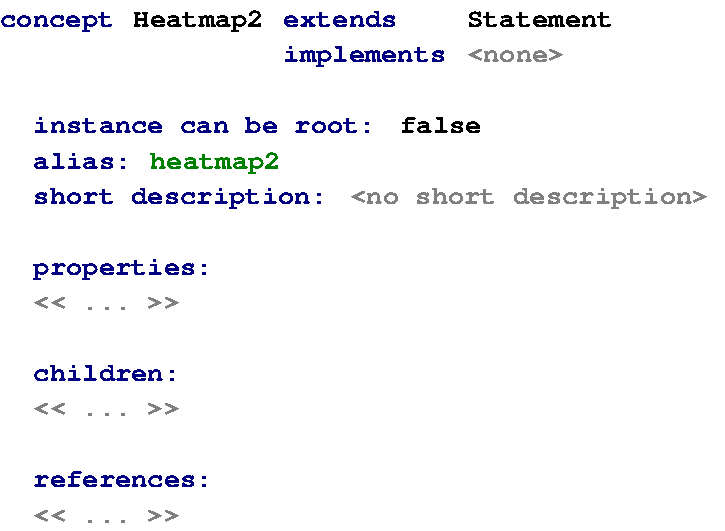
\includegraphics[width=\figWidthNarrow]{figures/Heatmap2Concept.pdf}
\caption[Heatmap2 Concept.]{\textbf{Heatmap2 Concept.} The \texttt{Heatmap2} concept extends Statement. When the language is composed with MetaR, \texttt{Heatmap2} will become available for auto-completion whenever a MetaR Statement can be used.}
\label{fig:Heatmap2Concept}
\end{figure}


\begin{figure}[htbp]
  \centering
  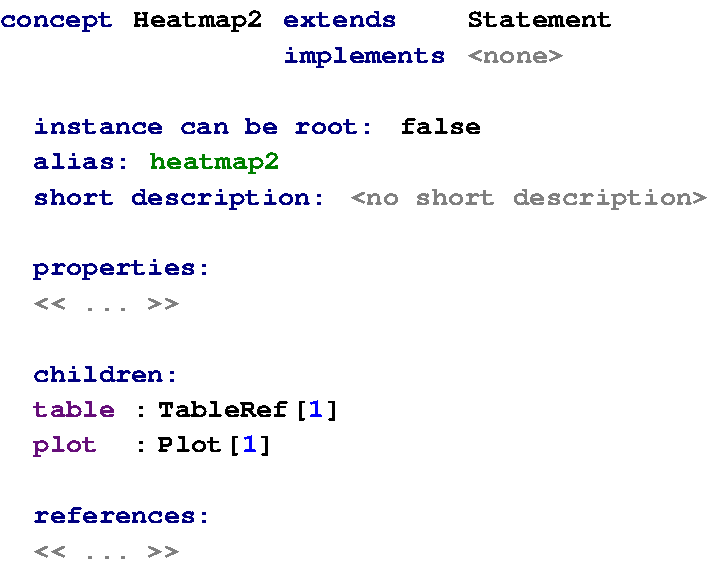
\includegraphics[width=\figWidthNarrow]{figures/Heatmap2Concept_Complete.pdf}
\caption[Complete Heatmap2 Concept.]{\textbf{Complete Heatmap2 Concept.} This figure shows the completed \texttt{Heatmap2} concept with an alias and children for table and plot.}
\label{fig:Heatmap2ConceptCompleted}
\end{figure}

Figure~\ref{fig:Heatmap2ConceptCompleted} presents the completed concept after adding alias, table and plot. 
\section{Define the Editor}
An MPS editor customizes how a node appears in the editor. Create an editor for \texttt{Heatmap2} (see~\cite{campagne2014mps}) and define its content as shown in Figure~\ref{fig:EditorForHeatmap2}.
\begin{SCfigure}
  \centering
  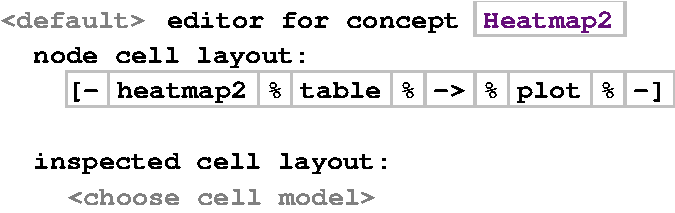
\includegraphics[width=\figWidthNarrow]{figures/EditorForHeatmap2.pdf}
\caption[Editor of the Heatmap2 Statement.]{\textbf{Editor of the Heatmap2 Statement.} Notice how the editor simply shows the name of the statement, delegates to the TableRef editor to render the table reference, and delegates to the Plot editor to show the plot child.}
\label{fig:EditorForHeatmap2}
\end{SCfigure}

\section{Generate R Code}
In order to generate the statement to R code, we will use the MPS Generator aspect. 

In the first step, we create a reduction rule, see Figure~\ref{fig:GeneratorHowToStep1} and~\cite{campagne2014mps} (Generator Aspect chapter). The rule indicates that nodes of the \texttt{Heatmap2} concept will be transformed with the \texttt{reduce\_Heatmap2} template. The template was created using the \textbf{New Template} intention found on the reduction rule node. See detailed instructions in~\cite{campagne2014mps}. When configuring the type of the output node (under \texttt{content node:}), use \texttt{Lines}, from the language \textit{org.campagnelab.textoutput} to produce text with the MPS Generator aspect.

\begin{figure}[h!tbp]
  \centering
  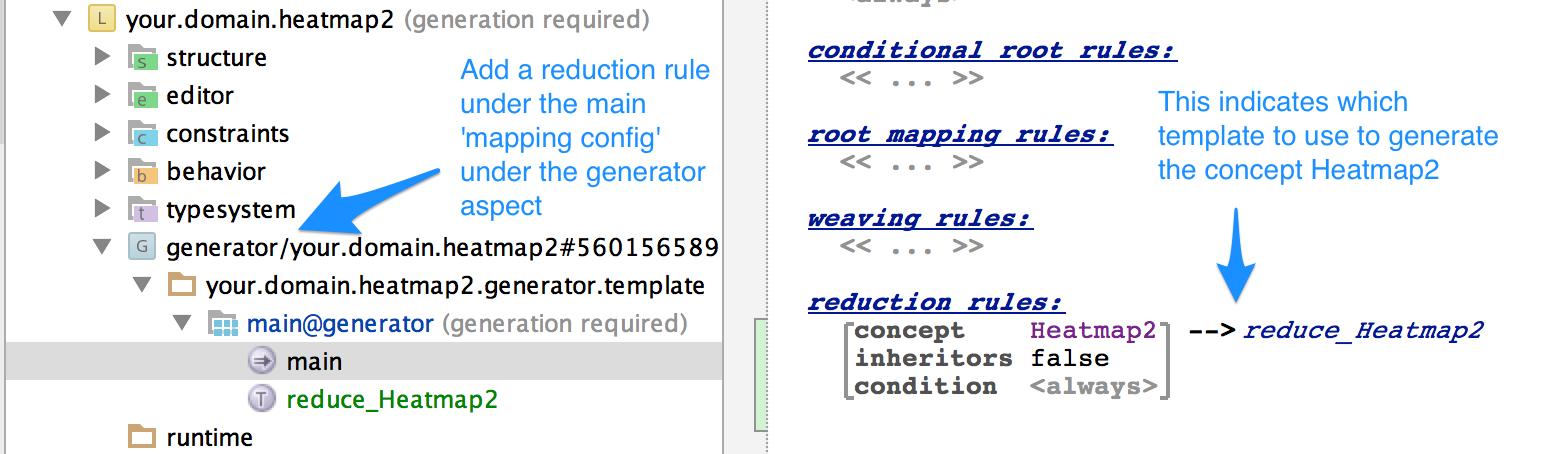
\includegraphics[width=\figWidthWide]{figures/GeneratorHowToStep1.png}
\caption[Generate R Code: Step 1.]{\textbf{Generate R Code: Step 1.} Start by adding a reduction rule.}
\label{fig:GeneratorHowToStep1}
\end{figure}

The simplest template we can build for the \texttt{Heatmap2} concept is shown on Figure~\ref{fig:SimplestTemplate}. Simply calling the \texttt{heatmap.2} function is a good start, but trying to run this will fail because the function is not part of a plain R distribution. The next section explains how to install the gplot R package which provides the function and activate it. 

\begin{figure}[h!tbp]
  \centering
  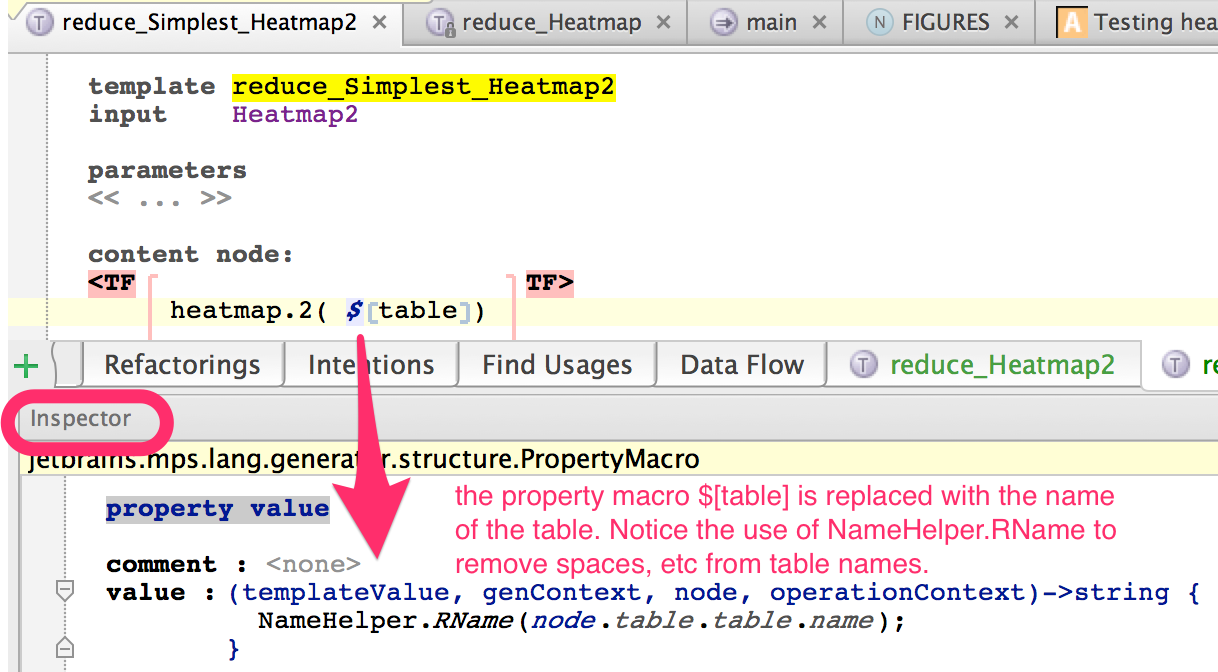
\includegraphics[width=\figWidthWide]{figures/SimplestTemplate.png}
\caption[Simplest template.]{\textbf{Simplest template.} The template simply converts any node of the \texttt{Heatmap2} concept to a line of R code that calls the \texttt{heatmap.2} function with the table as an argument. Notice the use of a property macro to obtain the R name of the table variable from the node table attribute. Open the \inspectorTabIcon{} to see what value the macro will take when a node is generated to R code.}
\label{fig:SimplestTemplate}
\end{figure}

\subsection{Adding package and library support}
MetaR makes it easy to install R packages as they are needed by an analysis. For this to work, we need to declare that the \texttt{Heatmap2} concept depends on the \textit{gplots} R package.  We can do this by overriding the default Statement behavior method called \texttt{dependencies()}. This method is expected to return the list of package names that must be installed and loaded before the statement can execute. To override the method, navigate to the \texttt{Heatmap2} concept in the editor, select the behavior tab, create the behavior and when the empty behavior is shown, select Override Behavior Method (see Figure~\ref{fig:CreateBehaviorAndOverride}).
Replace the body of the method with 
\begin{lstlisting}
return new singleton<string>("gplots");
\end{lstlisting}
Figure~\ref{fig:dependenciesMethodComplete} shows the complete  method. Rebuild the language, then the solution. When you run the Analysis, you will see that the gplots package is being installed:
\begin{lstlisting}
...
Loading required package: gplots
Installing package into '/Users/fac2003/.metaRlibs'
(as 'lib' is unspecified)
also installing the dependencies 'bitops', 'gtools', 'gdata', 
    'caTools'

trying URL ....
\end{lstlisting}

\begin{SCfigure}
  \centering
  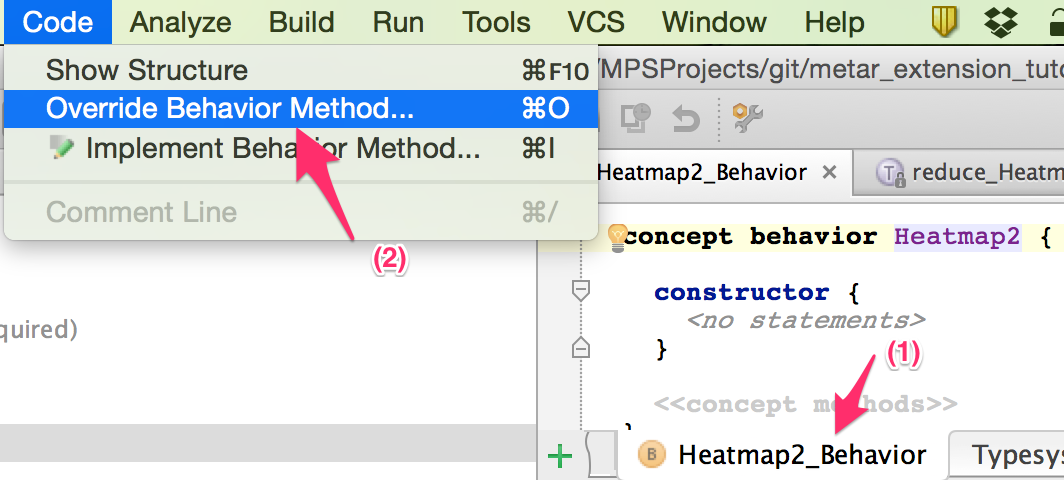
\includegraphics[width=\figWidthNarrow]{figures/CreateBehaviorAndOverride.png}
\caption[Override Behavior Methods.]{\textbf{Override Behavior Methods.} When the override dialog appear, choose dependencies() and click OK.}
\label{fig:CreateBehaviorAndOverride}
\end{SCfigure}


\begin{SCfigure}
  \centering
  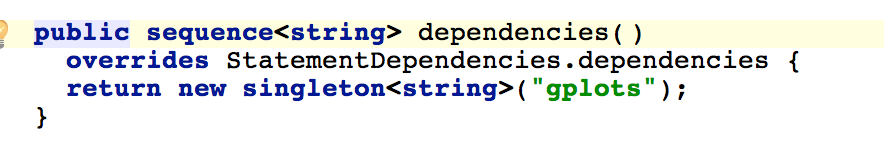
\includegraphics[width=\figWidthSmall]{figures/dependenciesMethodComplete.png}
\caption[Complete Dependencies Behavior Method.]{\textbf{Complete Dependencies Behavior Method.}}
\label{fig:dependenciesMethodComplete}
\end{SCfigure}

\subsection{Adjust Generator Priorities}
Adjust the generator priorities as shown in Figure~\ref{fig:Generator_Properties_your_domain_heatmap2}. To set priorities, you need to define a Design dependency on \textit{org.campagnelab.metar.tables} in the generator aspect Module Properties dialog. 

\begin{figure}[h!tbp]
  \centering
  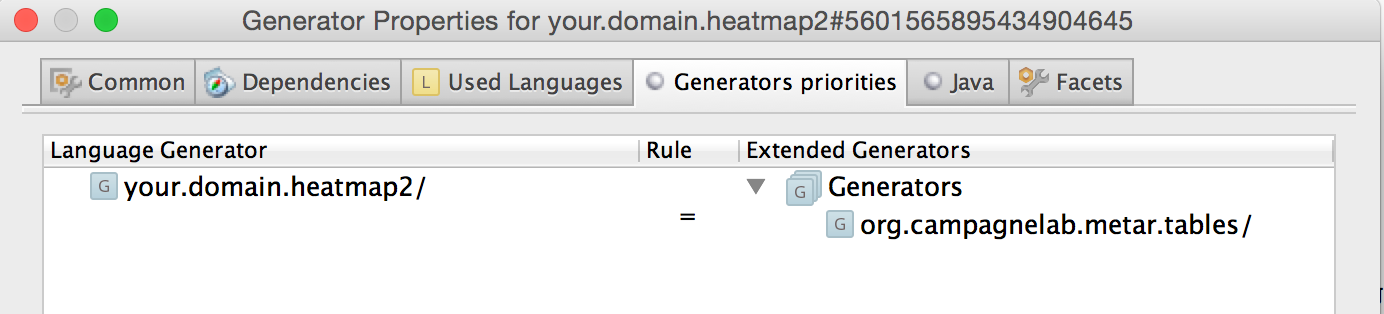
\includegraphics[width=\figWidthWide]{figures/Generator_Properties_your_domain_heatmap2.png}
\caption[Adjust Generator Priorities.]{\textbf{Adjust Generator Priorities.} Generation of the \texttt{Heatmap2} concept has to happen in the same generation phase as the generation of the  \textit{org.campagnelab.metar.tables} concepts. Failure to adjust priorities may result in table names not being correctly inserted in the \texttt{heatmap.2} function call.}
\label{fig:Generator_Properties_your_domain_heatmap2}
\end{figure}

\subsection{Redirecting the plot output}
The next problem with the simple template is that it fails to write the image of the plot in  location where MetaR can find it. This is needed to display the plot preview, or to make it possible to use plots with the \texttt{multiplot} statement.
The strategy we use to handle both cases is to wrap the actual plotting code inside a \texttt{plot\_xxx} function. The function is named with the id of the statement that generates the plot, so that we can easily refer to it in other places where the plot should be reused. We start by defining this function:

\begin{lstlisting}
plot_ $[id]=function(t){                        
  heatmap.2(as.matrix(t)) 
}                                             
\end{lstlisting}

The function accepts one argument: the name of the table to plot. 

\begin{remark}
The number of arguments is up to you, since you will generate both the function and the function calls.

\end{remark}

The next step is to add the R code for generating a PNG file with the plot to show a preview in the inspector. To this end, we redirect the plot output with png(), call the plot function, and close the graphics output (dev.off()):

\begin{lstlisting}
png(file=" $[plot.png]", width= $[w], height= $[h])
plot_ $id( $[table])                           
ignore <- dev.off()                          
\end{lstlisting}
Notice how the parameters of the png function are taken from the Plot node.
For instance, the \texttt{\$[plot.png]} macro will expand to 

\begin{lstlisting}
new RPath(node.plot.getPath()).toString();
\end{lstlisting}


\subsection{Handling errors}
Accurate error reporting is important to the end-user. When things do not go well and the R code fails, it is useful to know precisely which MetaR statement generated the error. In MetaR, this is done by taking advantage of the \texttt{tryCatch} R functions (see \url{http://mazamascience.com/WorkingWithData/?p=912}). 

Because \texttt{tryCatch} is not particularly intuitive and is rather verbose, MetaR extends the \textit{org.campagnelab.TextOutput} language with the \texttt{tryForNode} statement (concept name: \texttt{TryAndReport}). The \texttt{tryForNode} statement attempts to execute some lines of R code, and reports any errors that occur in these lines with a link to the statement that produced the error or warning. The \texttt{tryForNode} statement is also responsible for showing the \texttt{STATEMENT\_EXECUTED/\allowbreak{}8289224\allowbreak{}569309332962/} lines in the Run tool, which are hyperlinked to statements in the editor. 

The statement \texttt{tryForNode} takes an ID, which is the result of the \texttt{id()} method defined for each MetaR statement. The value of the ID can be set as usual with a property macro (its value should be \texttt{node.id()}). Figure~\ref{fig:Heatmap2GeneratorComplete} shows the completed template for \texttt{Heatmap2}. While the statement only needs to call the \texttt{heatmap.2} function, handling possible errors and producing plots that can be reused to build multi-panel figures have added quite a few lines to the output.
\begin{remark}
MetaR 1.3.1.1 makes it easier to wrap \textit{TextOutput} \texttt{Lines} into a \texttt{tryForNode} block. Select a node of type \texttt{Lines} (highlighted in blue braces) and invoke the intention \texttt{Wrap Lines in a TryForNode Block}. Note that this intention is not available for lines already inside a \texttt{tryForNode} block.
\end{remark}

\begin{figure}[h!tbp]
  \centering
  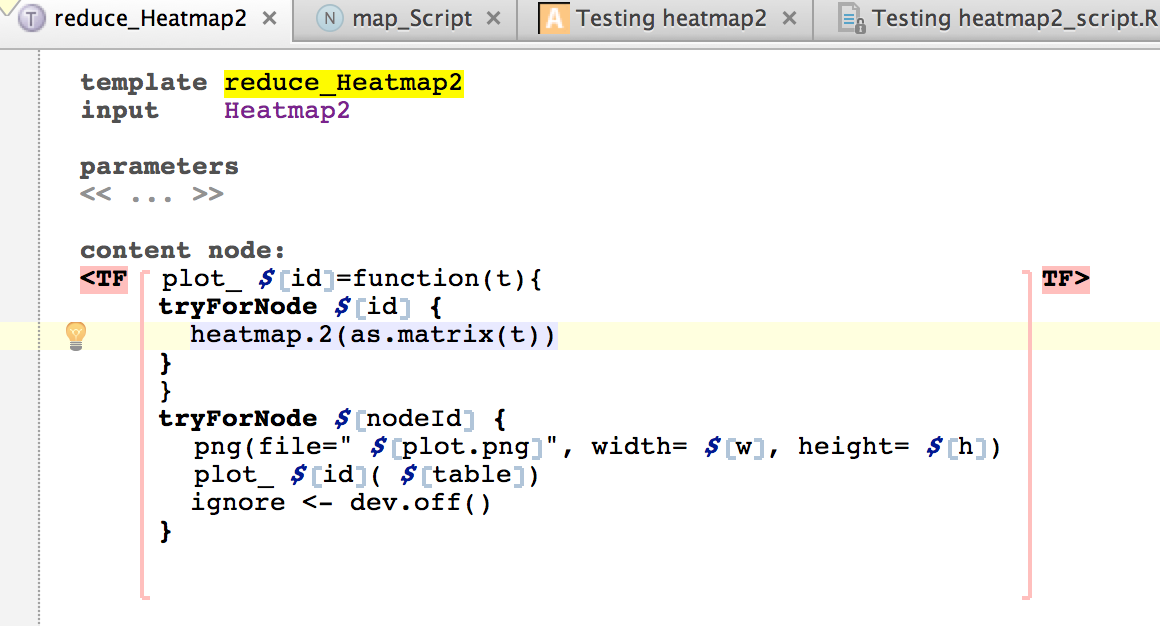
\includegraphics[width=\figWidthWide]{figures/Heatmap2GeneratorComplete.png}
\caption[Complete Generator for Heatmap2.]{\textbf{Complete Generator for Heatmap2.} This template wraps the \texttt{heatmap.2} function call inside a plot function (needed when building figures with multiple panels) and inside a \texttt{tryForNode} statement. The \texttt{tryForNode} statement generates to the \texttt{tryCatch} R language construct and appropriately reports errors to the end-user.}
\label{fig:Heatmap2GeneratorComplete}
\end{figure}
 
\section{Using the New Language}
Using the \textit{your.domain.heatmap2} language in MetaR analyses  requires adding the language under Used Languages, as shown here:

  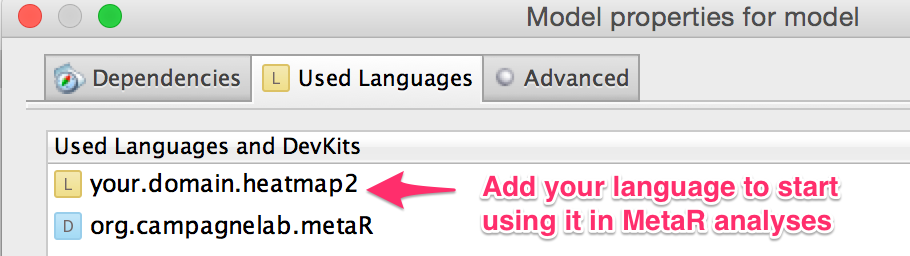
\includegraphics[width=\figWidthNarrow]{figures/LanguageExtensionUsedLanguages.png}

Once the language is added, you can create statements by typing the \texttt{Heatmap2} concept name. Figure~\ref{fig:Heatmap2_Execution} shows the result of using the new concept. 

\begin{figure}[h!tbp]
  \centering
  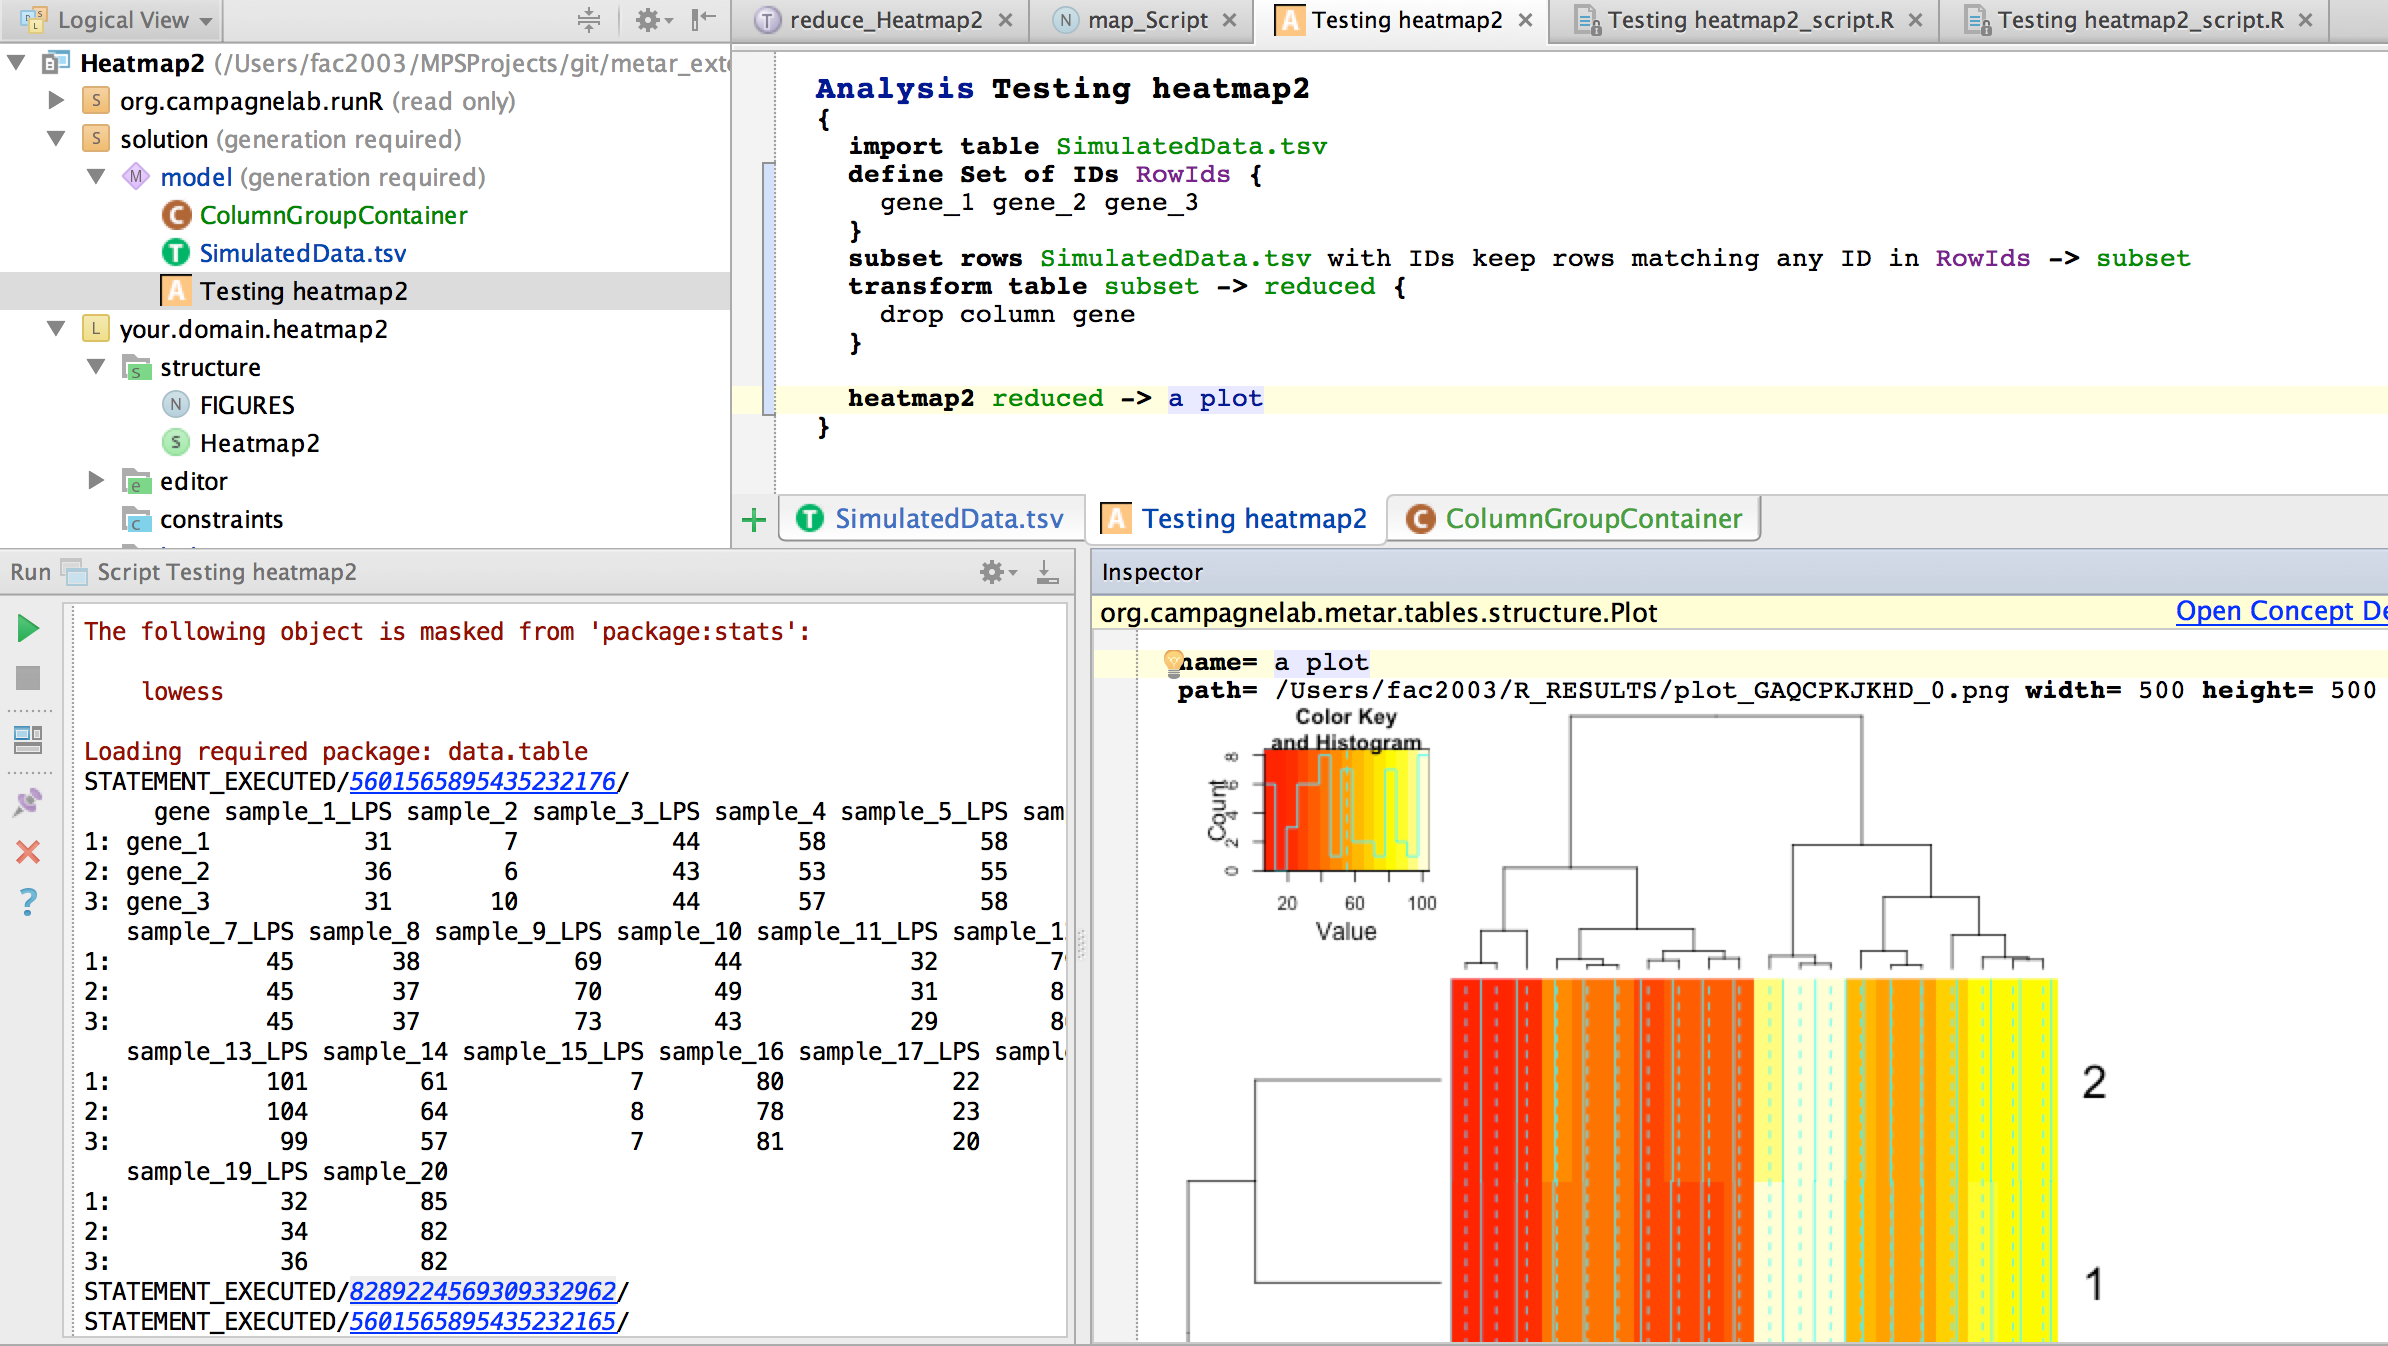
\includegraphics[width=\figWidthWide]{figures/Heatmap2_Execution.png}
\caption[Heatmap2 Execution.]{\textbf{Heatmap2 Execution.} This figure presents an Analysis using the new \texttt{Heatmap2} concept and shows the resulting plot preview in the inspector (bottom right). Error handling and progress indicators can be seen on the bottom left.}
\label{fig:Heatmap2_Execution}
\end{figure}



\section{Git Repository}\index{Git}
This concludes this tutorial. You can find a project with the \textit{heatmap2} language extension described in this Chapter at: \newline
\begin{flushright}
\texttt{https://bitbucket.org/\allowbreak{}campagnelaboratory\allowbreak{}/}\newline\texttt{metar\allowbreak{}\_extension\allowbreak{}\_tutorial}
\end{flushright}

